\documentclass[a4paper]{article}
%review 


%#########################################################################
\usepackage[utf8]{inputenc}
%\usepackage[T1]{fontenc}
%\usepackage[francais]{babel}
%\usepackage{lmodern}
\usepackage[hmargin=4cm, vmargin=2cm, includeheadfoot]{geometry}
\usepackage{alltt}
\usepackage{multicol}
\usepackage{amsmath,amssymb}
\usepackage{color}
\usepackage{graphicx}
\usepackage[francais,bloc,completemulti]{automultiplechoice}     % Mandatory for conversion



% exemple de commande utilisateur
\providecommand{\abs}[1]{\lvert#1\rvert}
%#########################################################################
% Entête
%#########################################################################



\title{Test de conversion AMC vers moodle}
\author{BN}



%#########################################################################
% Document
%#########################################################################
\begin{document}

%
% B A R E M E 
% e=incohérence; b=bonne; m=mauvaise; p planché (on ne descent pas en dessous)
\baremeDefautS{e=-0.5,b=1,m=-0.5}% never put b<1,
\baremeDefautM{e=-0.5,b=1,m=-0.25,p=-0.5}% never put b<1,




%question : environnement, text question
%element{label}{groupe} :commande, encapsule la commande pour lui donner un groupe
%reponses : environnement
%bonne  : commande
%mauvaise : commande
% B A R E M E 
% e=incohérence; b=bonne; m=mauvaise; p planché (on ne descent pas en dessous)
%\baremeDefautS{e=-0.5,b=1,m=-0.5}
%\baremeDefautM{e=-0.5,b=0.5,m=-0.25,p=-0.5}
% ajouter aucune de ces réponses n'est correcte
%\usepackage[francais,bloc,completemulti]{automultiplechoice}  

%===================================================================
% simple
\element{cat1}{
\begin{question}{Qsimple:img}    
On souhaite faire passer \textit{exactement}, par $N$ points donnés, un \texttt{polynôme} de degré \textbf{strictement} égal à $N-1$. Pour trouver les coefficients on doit résoudre un \emph{problème}
        \begin{center}
            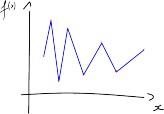
\includegraphics[width=0.5\textwidth]{./Figures/other/schema_interpL.png}
        \end{center}

  \begin{reponses}    
    \bonne{d'interpolation}
    \mauvaise{de moindre carré}
    \mauvaise{de Thelonius Sphere Monk 
        \begin{flushright}
                        
\includegraphics[height=2cm]{./Figures/tinymonk.pdf}
        \end{flushright}
        \begin{flushleft}
                        
\includegraphics[height=3cm]{./Figures/tinymonk.pdf}
        \end{flushleft}
    }
  \end{reponses}
\end{question}
}

%
%===================================================================
% questions à réponse multiple
% pas de bonne réponse, on doit ajouter un champ "aucune de ces réponses n'est correcte"
\element{cat1}{
\begin{questionmult}{Qmult:Aucune}  \bareme{e=-0.5,b=1,m=-1.,p=-0.5} % never put b<1,
Quel fruit possède un noyau?
  \begin{reponseshoriz}    
    \mauvaise{La pomme}
    \mauvaise{La tomate}
    \mauvaise{le Kiwi}
%    \mauvaise{En allant à $$ \int_0^2 x \mathrm{d} x $$ la ligne}
  \end{reponseshoriz}
\end{questionmult}
}
%
% il y a des bonne réponses et un tableau, verbatim, macro
\element{cat2}{
\begin{questionmult}{Qmult:TabVerbMacro}  
Quels sont les opérations qui donnent un chiffre présent dans le tableau?
    \begin{center}
        \begin{tabular}{ccc}
        \hline
	        12 & 2 & $2^3$ \\
	        \multicolumn{2}{c}{Deux} & 
\includegraphics[height=16pt]{./Figures/other/4.png} \\
	        \hline
        \end{tabular}
    \end{center}
  \begin{reponses}    
    \bonne{ Ou en \texttt{C} using \texttt{alltt} package
\begin{alltt}
int s=-2; \\
for (int i=0;i<4; i++)\{ \\
     s=i*i+s; \\
\} 	
\end{alltt}
%        \begin{verbatim}%L'environnement verbatim pose en effet des problèmes avec AMC
%            int s=0
%            for(int i;i=0; i<4){
%            	   s++
%            } 	               
%        \end{verbatim}
              }
    \bonne{$\abs{-10-2}$ (math inline and newcommand)}
    \mauvaise{la réponse en image 
\includegraphics[height=16pt]{./Figures/other/4r.png}}
    \mauvaise{$6\times 6$}
    \mauvaise{Avec une équation  $$ \int_0^2 x \mathrm{d} x $$ } % works
    \bonne{Avec une équation matricielle
        \begin{equation}
          \mathrm{det} \begin{pmatrix}1 & 2 \\ -1 & 10 \end{pmatrix} = \begin{vmatrix}1 & 2 \\ -1 & 10 \end{vmatrix}
        \end{equation}
    }
%    \mauvaise{Avec une autre équation utilisant \texttt{aligned} amsmath environnemnt
%            \begin{equation}\left\{\begin{aligned}\displaystyle t_{0}&amp;\displaystyle=1/\sqrt{3}\\&#10;\displaystyle t_{i+1}&amp;\displaystyle=\frac{\sqrt{t_{i}^{2}+1}-1}{t_{i}}\end{aligned}\right..
%            \end{equation}
%    }        
  \end{reponses}
\end{questionmult}
}


% test with englisg keywords
% example from http://home.gna.org/auto-qcm/auto-multiple-choice.en/latex.shtml#latex.simple
\element{english}{
\begin{question}{prez}    
  Among the following persons, which one has ever been a President of the French Republic?
  \begin{choiceshoriz}
    \correctchoice{René Coty}
    \wrongchoice{Alain Prost}
    \wrongchoice{Marcel Proust}
    \wrongchoice{with an image 
\includegraphics[height=16pt]{./Figures/other/4r.png}}
  \end{choiceshoriz}
\end{question}
}

\element{english}{
\begin{questionmult}{pref}     \scoring{e=-0.5,b=1,m=-.25,p=-0.5}
  Among the following cities, which ones are French prefectures?
  \begin{choices}
    \correctchoice{Poitiers}
    \wrongchoice{Sainte-Menehould}
    \correctchoice{Avignon}
  \end{choices}
\end{questionmult}
}

% #################################################################
% C R E A T I O N  D E S  C O P I E S
% #################################################################
\exemplaire{1}{    	% nombre de sujet différent

    %debut de l'en-tête des copies :    

    \vspace*{.5cm}
    \begin{minipage}{.4\linewidth}
	    \centering\large\bf Test
    \end{minipage}
    \champnom{\fbox{    
                    \begin{minipage}{.5\linewidth}
                      Nom et prénom :

                      \vspace*{.5cm}\dotfill
                      \vspace*{1mm}
                    \end{minipage}
             }}

    \begin{flushleft}
Certaine question peuvent sembler étrange, c'est le but !  
        \begin{center}
            \Large{\textsc{QCM using AMC Latex Format}}\\ 
            \normalsize
        \end{center}
    \end{flushleft}



    % mélange et catégorie (groupe dans ACM)
    \cleargroup{BigGroupe}
    \copygroup{cat1}{BigGroupe}
    \copygroup{cat2}{BigGroupe}
    \copygroup{english}{BigGroupe}
    \melangegroupe{BigGroupe}
    \restituegroupe{BigGroupe}
}   




\end{document}
